\documentclass[prb,preprint]{revtex4-1} 
% The line above defines the type of LaTeX document.
% Note that AJP uses the same style as Phys. Rev. B (prb).

\usepackage{amsmath}  % needed for \tfrac, \bmatrix, etc.
\usepackage{amsfonts} % needed for bold Greek, Fraktur, and blackboard bold
\usepackage{graphicx} % needed for figures
\usepackage{color}
\usepackage{ulem}
\begin{document}

% Be sure to use the \title, \author, \affiliation, and \abstract macros
% to format your title page.  Don't use lower-level macros to  manually
% adjust the fonts and centering.

\title{Single-Photon Interference}


\author{Liza Mulder}
\email{emulder@smith.edu}
\affiliation{Department of Physics, Smith College, Northampton, MA 01063}


\author{Isabel Lipartio}
\email{iliparti@smith.edu}
\affiliation{Department of Physics, Smith College, Northampton, MA 01063}


\date{\today}



\begin{abstract}



\end{abstract}

\maketitle % title page is now complete


\section{Introduction} % Section titles are automatically converted to all-caps.
% Section numbering is automatic.




\section{Methods}

We used the Teach-Spin "2-Slit Interference One Photon at a Time" Apparatus for this experiment.  The apparatus comes with a long black box containing an adjustable light source (with green filter to restrict wavelength and intensity), a 670nm laser source for alignment, four magnetic slit-holders along the length of the box for adding slits in the path of the light, and two detector options at the end: a photodiode (for laser light) and a photomultiplier tube (for lightbulb illumination).  We placed a single columnating slit in the first holder to focus the light from the lightbulb. This created vertical a single-slit diffraction pattern, which we centered on the next set of slits.  In the second slit holder, in the middle of the box, we placed the double-slit, and immediately following that we placed the slit blocker (a wide single-slit) so we could choose to allow light through one slit, both slits, or neither.  At the far end of the box we placed a single slit for the detector slit - by moving this slit holder lengthwise across the channel we could "scan" the interference pattern and measure photon counts at regular intervals.  

Behind the detector slit was a photomultiplier tube (PMT).  A PMT generates an electrical current


\begin{figure}[h!]
\centering
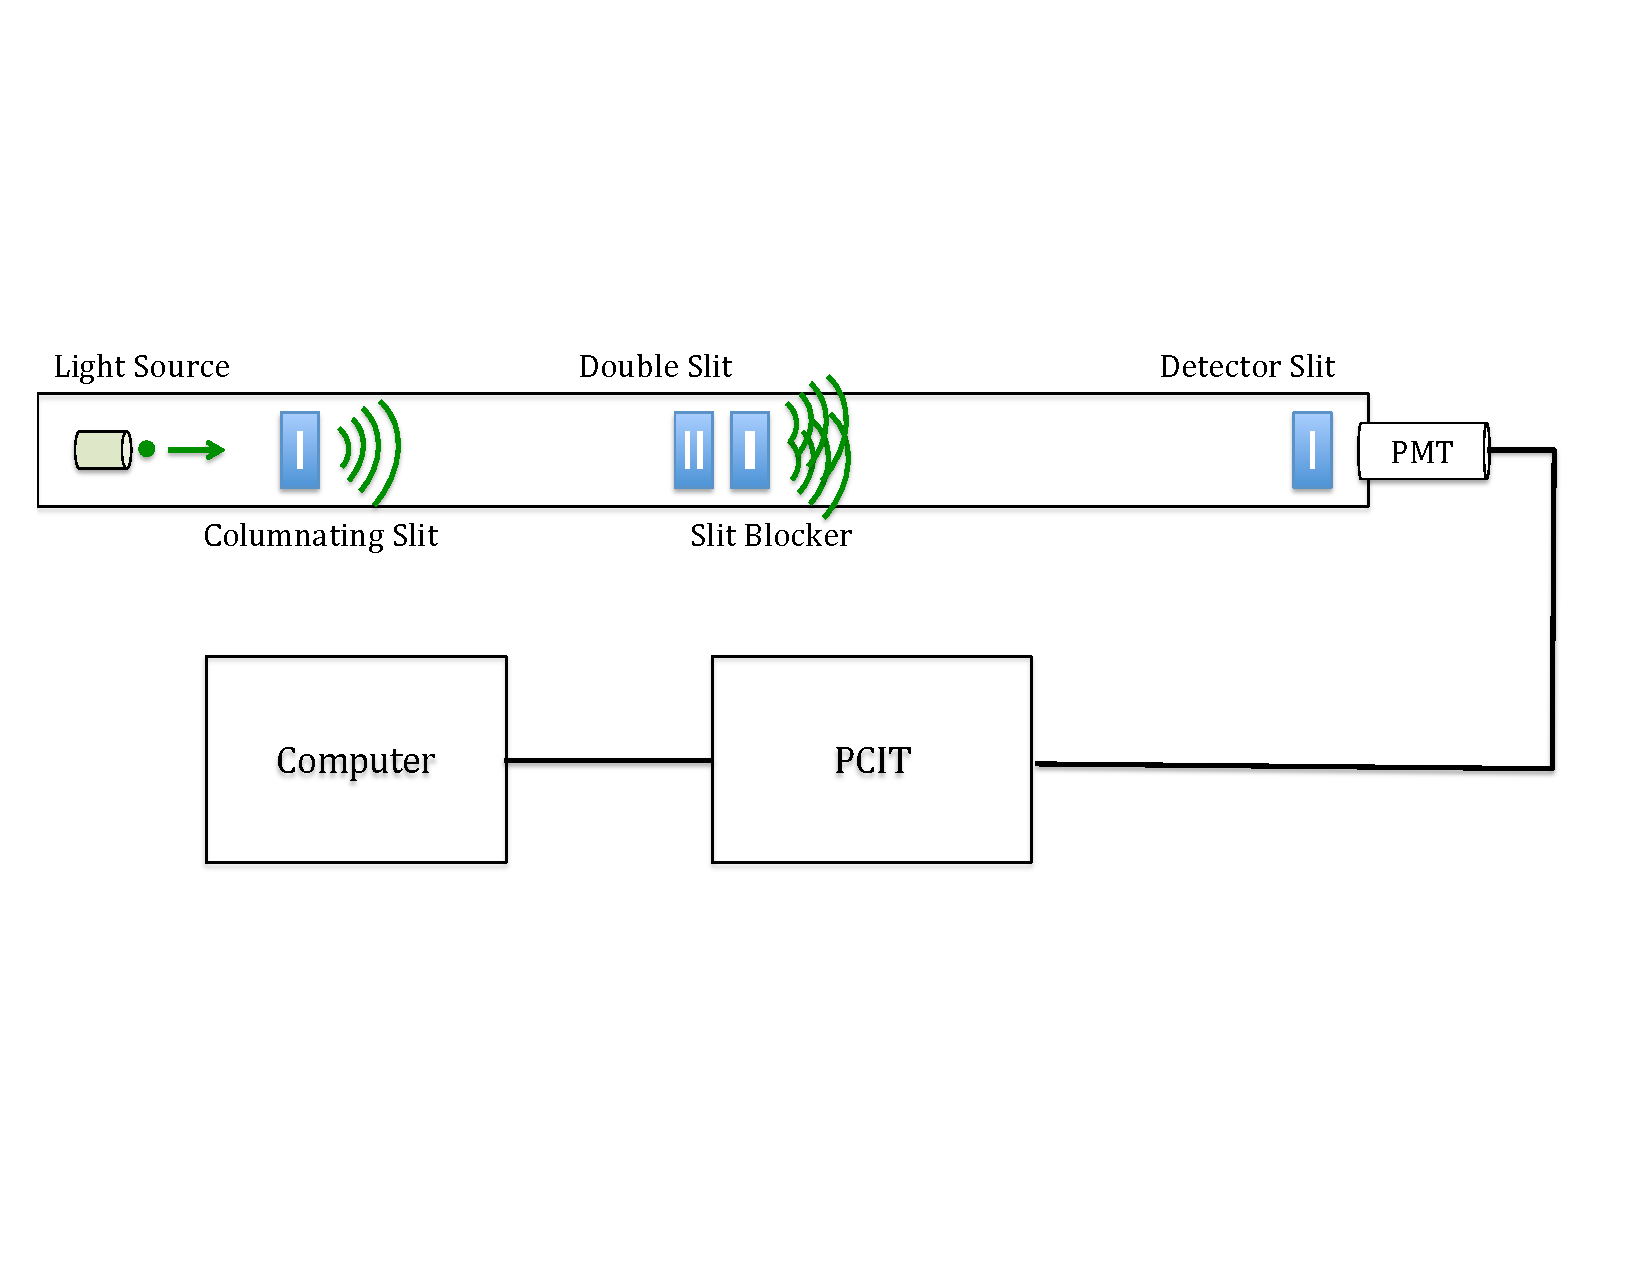
\includegraphics[width=6in]{set-up.pdf}
\caption{Teach-Spin apparatus to measure quantum interference: a 1m-long black box containing an adjustable light source (450nm), columnating single slit, double slit, slit blocker, detector slit, and photomultiplier tube (PMT) detector. We sent the PMT output to a pulse-counter interval timer (PCIT), and from there to the computer.}
\label{set-up}
\end{figure}





\section{Results}



\section{Analysis}



\section{Discussion}

\section{Conclusion}

 
\begin{thebibliography}{3}


\end{thebibliography}
\end{document}
